\documentclass{template}
\title{Accelerated Radiative Diffusion Problems\\
\normalsize Original article: Synthetic Acceleration for Radiative Diffusion Calculations~\cite{morel1985synthetic}}

\author{Kyle Hansen}
\date{NE 795 Computational Project\\
12 December 2025}

\usepackage{cancel}
\usepackage{xcolor}

\usepackage{float}

\usepackage{algpseudocode}
\usepackage{algorithm}
\usepackage{subcaption}

\usepackage{dirtree}

\newcommand*\Let[2]{\State{#1 $\gets$ #2}}
\algrenewcommand\algorithmicrequire{\textbf{Precondition:}}
\algrenewcommand\algorithmicensure{\textbf{Postcondition:}}


\newcommand*\multbox[1]{\fbox{\hspace{0ex}#1\hspace{0ex}}}

\newcommand{\I}{\mathcal{I}}
\newcommand{\E}{\mathcal{E}}

\definecolor{base03}{HTML}{002b36}
\definecolor{bg-light}{rgb}{0.95, 0.95, 0.95}

\newminted{python}{style=lightbulb, bgcolor=base03}
\newmintinline{python}{style=xcode, bgcolor=bg-light}

\begin{document}

\maketitle

\section{Problem}

The equations for radiative diffusion are 

\begin{subequations}\label{eq:radiative-diffusion}
    \begin{gather}
    \label{eq:spectral_diffusion}
  \frac{1}{c}\frac{\partial I}{\partial t} - \nabla \cdot D(\nu) \nabla I(\nu) + \rho \kappa(E)I(E) = \rho\kappa(\nu)\beta(\nu, T)\\
  \label{eq:spectral_temperature}
  \rho C_v \frac{\partial T}{\partial t} = \nabla \cdot K \nabla T - \nabla {\mathbb{P}u} + \rho \int_0^\infty \kappa(E^\prime)\left[ I(E^\prime) - \beta(E^\prime, T) \right] dE^\prime + Q,
\end{gather}
\end{subequations}


where \autoref{eq:spectral_diffusion} is the radiative diffusion equation, where $c$ is the speed of light, $I$ is scalar intensity $I_{\nu}(x) = \int_{4\pi} \I_\nu(x,\Omega) d\Omega = cE$, $D$ is the radiative diffusion constant $(3\rho\kappa)^{-1}$, $\kappa$ is specific opacity $[\text{cm}^2/\text{g}]$, and $\beta$ is the angle-integrated Planck function, $\beta_\nu(T) = \int_{4\pi} B_\nu(T)d\Omega$.

\autoref{eq:spectral_temperature} is the heat diffusion equation with radiation and hydrodynamic effects, where $\rho$ is material density, $C_v$ is material heat capacity, $K$ is thermal conductivity, $\mathbb{P}$ is the fluid pressure tensor, $u$ is fluid velocity, and $Q$ is heat generation per unit mass.

The energy domain can be discretized using $N_g$ energy groups $G_i = [\nu_{i}, \nu_{i+1}]$ such that $\nu_0 = 0$ and $\nu_{N_g + 1} = \infty$. Using this discretization, and using $\varkappa = \rho\kappa$, the diffusion equations become

\begin{subequations}
    \begin{gather}
  \frac{1}{c}\frac{\partial I_k}{\partial t} - \nabla \cdot D_k \nabla I_k + \varkappa_k I_k = \varkappa_k \beta_k(T)\\
  \rho C_v \frac{\partial T}{\partial t} = \nabla \cdot K \nabla T - \nabla {\mathbb{P}u} +  \sum_{g=1}^{N_g} \varkappa_g\left[ I_g - \beta_g(T) \right]^\prime + Q,
\end{gather}
\end{subequations}

where

\begin{subequations}
    \begin{align}
    I_k &= \int_{G_k} I(\nu) d\nu\\
    \beta_k &= \int_{G_k} \beta(\nu, T) d\nu\\
    D_k\nabla I_k &= \int_{G_k}D(\nu)\nabla I(\nu)d \nu\\
    \varkappa_k &= \frac{\int_{G_k} \left[\beta(\nu) - I(\nu) \right]   \varkappa(\nu) d\nu}{\int_{G_k} \left[\beta(\nu) - I(\nu) \right] d\nu}.
\end{align}
\end{subequations}

Discretizing in time using Backward Euler (time index $n$), with lagged coefficients, \autoref{eq:radiative-diffusion} becomes:

\begin{subequations}
    \begin{gather}
    \frac{1}{c}\frac{I^{n+1} - I^n}{\Delta t^n} - \nabla \cdot D_k^n \nabla I_k^{n+1} + \varkappa_k^n I_k^{n+1} = \varkappa_k^n \beta_k\left(T^{n+1}\right); \qquad k=1\dots N_g\\
    \rho C_v^n \frac{T^{n+1} - T^n}{\Delta t^n} = \nabla \cdot K^n \nabla T^{n+1} - \nabla {\mathbb{P}u} +  \sum_{g=1}^{N_g} \varkappa_g^n \left[ I_g^{n+1} - \beta_g(T^{n+1}) \right] + Q^{n+1}.
\end{gather}
\end{subequations}


The time-advanced Planck function $\beta$ is approximated using the first-order Taylor expansion $\beta(T^{n+1}) \approx \beta(T^n) + \frac{\partial \beta}{\partial T} (T^{n+1} - T^n)$, which leads to the system for $T^{n+1}$ and $I^{n+1}$,

\begin{subequations}
   \begin{gather}
    \frac{1}{c}\frac{I^{n+1} - I^n}{\Delta t^n} - \nabla \cdot D_k^n \nabla I_k^{n+1} + \varkappa_k^n I_k^{n+1} = \varkappa_k^n  \left(\beta(T^n) + \frac{\partial\beta}{\partial T} \Delta T^{n+1} \right)    ; \qquad k=1\dots N_g\\
    \rho C_v^n \frac{\Delta T^{n+1}}{\Delta t^n} = \nabla \cdot K^n \nabla T^{n+1} - \nabla {\mathbb{P}u} +  \sum_{g=1}^{N_g} \varkappa_g^n \left[ I_g^{n+1} - \beta(T^n) - \frac{\partial\beta}{\partial T} \Delta T^{n+1} \right] + Q^{n+1}.
\end{gather}
\end{subequations}

Finally, the temperature operator is split into the hydrodynamic and radiative contributions,

\begin{subequations}
    \begin{gather}
       \label{eq:rad-temperature}\rho C_v^n \frac{\Delta T^{n+1}}{\Delta t^n}  = \nabla \cdot K^n \nabla T^{n+1} - \nabla {\mathbb{P}u} +  Q^{n+1}\\
    \label{eq:needs-dt}\frac{1}{c}\frac{I^{n+1} - I^n}{\Delta t^n} - \nabla \cdot D_k^n \nabla I_k^{n+1} + \varkappa_k^n I_k^{n+1} = \varkappa_k^n  \left(\beta(T^n) + \frac{\partial\beta}{\partial T} \Delta T^{n+1} \right)    ; \qquad k=1\dots N_g\\
    \rho C_v^n \frac{\Delta T^{n+1/2}}{\Delta t^n} =   \sum_{g=1}^{N_g} \varkappa_g^n \left[ I_g^{n+1} - \beta(T^n) - \frac{\partial\beta}{\partial T} \Delta T^{n+1/2} \right],
\end{gather}
\end{subequations}

where $T^{n+1} = T^n + \Delta T^{n+1/2} + \Delta T^{n+1}$. The indices $n+1/2$ and $n+1$ in this case refer to two separate contributions in the same time step, not temperature change at an intermediate time step.

\autoref{eq:rad-temperature} can be immediately solved for temperature change,

\begin{equation}\label{eq:temperature-change}
    \Delta T^{n+1/2} = \frac{\sum_{g=1}^{N_g} \varkappa_g \left[ I_g^{n+1} - \beta_g^n \right] + Q}{\frac{\rho C_v^n}{\delta t^n} + \sum_{g=1}^{N_g} \varkappa_g \frac{\partial \beta}{\partial T}},
\end{equation}

which is then substituted into \autoref{eq:needs-dt} to give the radiative diffusion with implicit $\Delta T$:
\begin{subequations}
\begin{equation}\label{eq:standard_diffusion}
  \frac{1}{c \Delta t^n}\left( I^{n+1} - I^n \right)- \nabla \cdot D_k^n \nabla I_k^{n+1} + \varkappa_k^n I_k^{n+1} = \eta \chi_k  \sum_{g=1}^{N_g}\varkappa_g I_g^{n+1} + q_k
\end{equation}

where
  \begin{align}
    \eta   &=  \left[\sum_{g=1}^{N_g}\varkappa_g\frac{\partial \beta_g}{\partial T}\right] \cdot {\left[ \frac{\rho C_v}{\Delta t^n} + \sum_{g=1}^{N_g}\varkappa_g\frac{\partial \beta_g}{\partial T} \right]}^{-1} \\
    \chi_k &=  \left[ \varkappa_k  \frac{\partial \beta_k}{\partial T}   \right] \cdot {\left[\sum_{g=1}^{N_g}\varkappa_g\frac{\partial \beta_g}{\partial T}\right]}^{-1}\\
    q_k    &=  \varkappa_k \beta_k  +  \eta \chi_k \left[ Q -  \sum_{g=1}^{N_g}\varkappa_g\frac{\partial \beta_g}{\partial T} \right].
  \end{align}
\end{subequations}

\autoref{eq:standard_diffusion} is solved for intensity, then temperature change is recovered afterward. This can be rearranged to further resemble a steady-state neutron diffusion equation,

    \begin{equation}
  \label{eq:neutron_diffusion}-\nabla \cdot D_k \nabla I_k^{n+1} + \left( \sigma_a + \sigma_{f, k} \right)I_k^{n+1} = \eta \chi_k \sum_{g=1}^{N_g}\sigma_{f, g}I_g^{n+1} + S_k
    \end{equation}

where

\begin{subequations}\label{eq:neutron_xs}
  \begin{align}
  \sigma_a     &= \frac{1}{c\Delta t^n}\\
  \sigma_{f, k} &= \varkappa_k\\
  S_k &= q_k + \frac{I_k^n}{c\Delta t^n}.
\end{align}
\end{subequations}

Here $\sigma_{f, k} = \varkappa_k$ acts as a fission cross section, where photons are re-emitted with the ``fission'' spectrum $\chi_k$, with multiplicity $\eta$, and capture cross section $\sigma_a$. The physical interpretation is that photons may be lost to material absorption or streaming in time (from $\frac{d}{dt}$). Those photons absorbed in the material are either re-emitted in the same time step, or contribute to temperature gain in the material.

The intensity equation is solved using power iteration on the fission source. Starting from initial iterate $I_k^{(0)}$, the $l+1$ iterate for intensity at the $n+1$ time step is found by solving the linear system

\begin{equation}\label{eq:iterative_neutron}
  -\nabla \cdot D_k \nabla I_k^{l+1} + \left( \sigma_a + \sigma_{f, k} \right)I_k^{l+1} = \eta \chi_k \sum_{g=1}^{N_g}\sigma_{f, g}I_g^l + S_k.
\end{equation}

The full iterative algorithm is displayed in \autoref{alg:unaccelerated}.



\begin{algorithm}
    \caption{Unaccelerated Iteration Algorithm}\label{alg:unaccelerated}
  \begin{algorithmic}[0]
    % \Require{$x$ and $y$ are packed dna strings of equal length $n$}
    \Statex{}
    \While{$t^n \leq t^{end}$}
      \Let{$n$}{$n+1$}
      \State{Compute (lagged) temperature-dependent coefficients using $T\vert_{t=t^{n-1}}$}
      \While{$\norm{I^{(l)} - I^{(l-1)}} > \epsilon\norm{I^{(l-1)}}$}
        \Let{$l$}{$l+1$}
        \Let{$I_k^{(l+1/2)}$}{Source iteration on $\eta\chi_k \sum_{g=1}^{N_g}\sigma_{f, g}I_g^{n+1}$ (\ref{eq:iterative_neutron})}
      \EndWhile{}
      \Let{$I_k^{n}$}{$I_k^{(l+1)}$}
      \State{Recover $\Delta T^{n+1/2}$ from $I_k^{n}$ (\ref{eq:temperature-change})}
      \If{$K \neq 0 \land u \neq 0$}
        \State{Solve thermal diffusion equation for $\Delta T^{n+1}$}
      \EndIf{}
      \Let{$T^{n+1}$}{$T^n + \Delta T^{n+1/2} + \Delta T^{n+1}$}
    \EndWhile{}
  \end{algorithmic}
\end{algorithm}



\subsection{Synthetic Acceleration Method}

The equation for exact multigroup error of the $l$th iterate (\autoref{eq:iterative_neutron}) is

\begin{equation}
  \label{eq:error-diffusion-equation}-\nabla \cdot D_k\nabla \epsilon_k^{l} + \left(\sigma_a + \sigma_{f, k}\right)\epsilon_k^{l} = \eta \chi_k \sum_{g=1}^{N_g} \sigma_{f, g} \left[ \epsilon_g^{l} +I_g^{l} - I_g^{l-1} \right].
\end{equation}

At equilibrium, this becomes

\begin{equation}
  \left(\sigma_a + \sigma_{f, k} \right)\epsilon_k^l = \eta\chi_k \sum_{g=1}^{N_G}\sigma_{f, g}\epsilon_g^l + \eta\chi_k \sum_{g=1}^{N_G}\sigma_{f, g}\left(I_g^l - I_g^{l-1} \right)
\end{equation}

and the group spectrum of $\epsilon$ is

\begin{equation}\label{eq:spectrum}
    \frac{\epsilon_k^l}{\E^l} = \frac{\langle \sigma_t \rangle \chi_k}{\sigma_{t, k}}
\end{equation}

where

\begin{subequations}
    \begin{align}
        \E^l &= \sum_{g=1}^{N_g}\epsilon_g^l\\
        \langle \sigma_t \rangle &= {\left[\sum_{g=1}^{N_g} \frac{\chi_g}{\sigma_{t, g}} \right]}^{-1}.
    \end{align}
\end{subequations}

Then, all groups of \autoref{eq:error-diffusion-equation} are summed, using this spectrum, to get

\begin{equation}
    \label{eq:correction}-\nabla \cdot \left[\langle D \rangle \nabla \E^l     +  \langle D^\prime \rangle  \E^l    \right]  + \E^l \left[\sigma_a + \langle \sigma_f \rangle (1 - \eta)\right] =  \eta  r^l
\end{equation}

where

\begin{subequations}
 \begin{align}
  \langle D \rangle &= \sum_{k=1}^{N_g}D_k \frac{ \langle \sigma_t \rangle \chi_k}{\sigma_{t, k}}  \\
  \langle D^\prime \rangle &= \sum_{k=1}^{N_g} D_k  \nabla   \frac{ \langle \sigma_t \rangle \chi_k}{\sigma_{t, k}}\\
  \langle \sigma_f \rangle &= \langle \sigma_t \rangle \sum_{g=1}^{N_g} \frac{\chi_g \sigma_{f, g}}{\sigma_{t, g}}\\
  r^{l+1/2} &= \sum_{g=1}^{N_g} \sigma{f, g} \left( I_g^{l+1/2} - I_g^l\right).
\end{align} 
\end{subequations}

Then the spectrum from \autoref{eq:spectrum} can be used to calculate the groupwise correction terms from the grey correction in \autoref{eq:correction}. The accelerated iterative scheme becomes

\begin{subequations}
    \begin{gather}
  \label{eq:diffusion-half-iter}-\nabla \cdot D_k \nabla I_k^{l+1} + \left( \sigma_a + \sigma_{f, k} \right)I_k^{l+1} = \eta \chi_k \sum_{g=1}^{N_g}\sigma_{f, g}I_g^l + S_k\\
  \label{eq:onegroup-error-iter}-\nabla \cdot \left[\langle D \rangle \nabla \E^{l+1/2}      +  \langle D^\prime \rangle  \E^{l+1/2}    \right]  + \E^{l+1/2}  \left[\sigma_a + \langle \sigma_f \rangle (1 - \eta)\right] =  \eta  r^{l+1/2} \\
  \label{eq:fix-diffuion}I^{l+1} = I_k^{l+1} + \E^{l+1/2}\frac{\langle \sigma_t \rangle \chi_k}{\sigma_{t, k}}
\end{gather}
\end{subequations}


The accelerated iterative algorithm is displayed in \autoref{alg:accelerated}



\begin{algorithm}[H]
    \caption{Accelerated Iteration Algorithm}\label{alg:accelerated}
  \begin{algorithmic}[0]
    % \Require{$x$ and $y$ are packed dna strings of equal length $n$}
    \Statex{}
    \While{$t^n \leq t^{end}$}
      \Let{$n$}{$n+1$}
      \State{Compute (lagged) temperature-dependent coefficients using $T\vert_{t=t^{n-1}}$}
      \While{$\norm{I^{(l)} - I^{(l-1)}} > \epsilon\norm{I^{(l-1)}}$}
        \Let{$l$}{$l+1$}
        \Let{$I_k^{(l+1/2)}$}{Source iteration on $\eta\chi_k \sum_{g=1}^{N_g}\sigma_{f, g}I_g^{n+1}$, using (\ref{eq:diffusion-half-iter})}
        \Let{$r^{(l+1/2)}$}{$\sum_{g=1}^{N_g} \sigma{f, g} \left( I_g^{l+1/2} - I_g^l\right)$}
        \Let{$\E^l$}{Grey correction equation using (\ref{eq:onegroup-error-iter})}
        \Let{$I_k^{(l)}$}{$I_k^{(l+1/2)} + \E^{l+1/2}\frac{\langle \sigma_t \rangle \chi_k}{\sigma_{t, k}}$ using (\ref{eq:fix-diffuion})}
      \EndWhile{}
      \Let{$I_k^{n}$}{$I_k^{(l+1)}$}
      \State{Recover $\Delta T^{n+1/2}$ from $I_k^{n}$}
      \If{$K \neq 0 \land u \neq 0$}
        \State{Solve thermal diffusion equation for $\Delta T^{n+1}$}
      \EndIf{}
      \Let{$T^{n+1}$}{$T^n + \Delta T^{n+1/2} + \Delta T^{n+1}$}
    \EndWhile{}
  \end{algorithmic}
\end{algorithm}






\section{Numerical Implementation}

Using the multigroup diffusion equation with Backward Euler, lagged coefficients, and implicit temperature to approximate a 1D thermal radiative transfer (TRT) problem gives, at each time step, \autoref{eq:iterative_neutron} can be split into two first-order ODEs,

\begin{subequations}\label{eq:mg-diffusion}
    \begin{gather}
        \frac{\partial F_k^{n+1}}{\partial x}  + \left( \sigma_a + \sigma_{f, k} \right)I_k^{l+1} = \eta \chi_k \sum_{g=1}^{N_g}\sigma_{f, g}I_g^l + S_k\label{eq:mg-diffusion-zeroth-moment}\\
        F_k^{n+1} = -D_k \frac{\partial I_k^{n+1}}{\partial x}\label{eq:mg-diffusion-first-moment}\\
        0 \leq x \leq X, \qquad k = 1,\hdots, N_g\notag
    \end{gather}
\end{subequations}


where temperature is recovered using \autoref{eq:temperature-change}. Boundary conditions for these equations are given by

\begin{gather}
    I^+(0) = I_{in}^+\\
    I^-(X) = I_{in}^-\\
    F^+(0) = F_{in}^+\\
    F^-(X) = F_{in}^-
\end{gather}

where 

\begin{gather}
    I^\pm = \pm \int_0^{\pm 1} \I(\mu)d\mu   \\
    F^\pm = \pm \int_0^{\pm 1} \mu \I(\mu)d\mu  
\end{gather}

First, the spatial domain is divided into $N_x$ cells $K_i = [x_{i-1/2}, x_{i+1/2}]; i=1,\hdots,N_x$, where $x_{1/2} =0$ and $x_{N_x + 1/2} = X$, and in each cell $K_i$ the width is $\Delta x_i = x_{i+1/2} - x_{i-1/2}$. Then, if temperature (and temperature-dependent coefficients) are taken to be constant within each cell, then, in the accelerated correction equation, the term $\langle D^\prime \rangle$ becomes zero, and the grey correction equation has the same form as \autoref{eq:mg-diffusion}, so they may be solved in the same way.

\subsection{LD Formulation}

First, $I$ and $F$ (and the source $S_k$) from \autoref{eq:mg-diffusion} are assumed to take the form

\begin{subequations}\label{eq:assumed-forms}
    \begin{gather}
        I(x) = I_{L, i} b_{L, i} + I_{R, i} b_{R, i}\\
        F(x) = F_{L, i} b_{L, i} + F_{R, i} b_{R, i}\\
        S(x) = S_{L, i} b_{L, i} + S_{R, i} b_{R, i}\\
        b_{L, i} = \frac{x_{i+1/2} - x}{\Delta x_i}, \qquad b_{R, i} = \frac{x - x_{i-1/2}}{\Delta x_i}
    \end{gather}
\end{subequations}

where the multigroup index $k$ and the time index $n$ have been omitted without loss of generality. The weak form of \autoref{eq:mg-diffusion} is found by multiplying by the test functions $b_{L, i}$ and $b_{R, i}$ and integrating over the cell.

\begin{subequations}
    \begin{multline}
        \int_{x_{i-1/2}}^{x_{i+1/2}}\frac{d F^{l+1}}{d x}b_{c, i} dx  + \left( \sigma_a + \sigma_{f} \right)\int_{x_{i-1/2}}^{x_{i+1/2}}I^{l+1} b_{c, i} dx =\\
         \eta \chi \sum_{g=1}^{N_g}\sigma_{f, g}\int_{x_{i-1/2}}^{x_{i+1/2}}I^{(l)}_g b_{c, i}dx + \int_{x_{i-1/2}}^{x_{i+1/2}}S b_{c, i}dx
    \end{multline}
    \begin{equation}
        \int_{x_{i-1/2}}^{x_{i+1/2}}F^{l+1}b_{c, i}dx = -D \int_{x_{i-1/2}}^{x_{i+1/2}}\frac{d I^{l+1}}{d x}b_{c, i}dx
    \end{equation}
    \begin{equation}
        c = L, R; \qquad i=1,\hdots, N_x \notag
    \end{equation}
\end{subequations}

or, rewriting the $\frac{d}{dx}$ terms using integration by parts,

\begin{subequations}
    \begin{multline}
        \left[F^{l+1} b_{c, i} \right]_{x-1/2}^{x+1/2} - \int_{x_{i-1/2}}^{x_{i+1/2}}\frac{d  b_{c, i}}{d x}F^{l+1} dx  + \left( \sigma_a + \sigma_{f} \right)\int_{x_{i-1/2}}^{x_{i+1/2}}I^{l+1} b_{c, i} dx =\\
         \eta \chi \sum_{g=1}^{N_g}\sigma_{f, g}\int_{x_{i-1/2}}^{x_{i+1/2}}I^{(l)}_g b_{c, i}dx + \int_{x_{i-1/2}}^{x_{i+1/2}}S b_{c, i}dx
    \end{multline}
    \begin{equation}
        \int_{x_{i-1/2}}^{x_{i+1/2}}F^{l+1}b_{c, i}dx = -D \left( \left[I^{l+1} b_{c, i} \right]_{x_{i-1/2}}^{x_{i+1/2}} -   \int_{x_{i-1/2}}^{x_{i+1/2}}\frac{d b_{c, i} }{d x}  I^{l+1} dx    \right)
    \end{equation}
    \begin{equation}
        c = L, R; \qquad i=1,\hdots, N_x. \notag
    \end{equation}
\end{subequations}

Using the assumed forms in \autoref{eq:assumed-forms} and the interface conditions

\begin{gather}
    I^b(x_{i+1/2}) = I^+ + I^-  = \frac{1}{2}\left(I_{R, i} + I_{L, i+1} \right) + \frac{3}{4}\left(F_{R, i} - F_{L, i+1} \right)\\
    F^b(x_{i+1/2}) = F^+ + F^- = \frac{1}{4} \left(I_{R, i} - I_{L, i+1} \right) + \frac{1}{2}\left(F_{R, i} + F_{L, i+1} \right)
\end{gather}

the local equations on the interior become,

\begin{multline}
    \frac{1}{4} \left(I_{L, i}^{(l+1)} - I_{R, i-1}^{(l+1)} \right) + \frac{1}{2}\left(F_{R, i}^{(l+1)} - F_{R, i-1}^{(l+1)} \right) + \frac{\sigma_t \Delta x_i}{6} \left( m_{LL} I_{L, i}^{(l+1)} + m_{LR}I_{R, i}^{(l+1)}\right) =\\
    \eta \chi \sum_{g=1}^{N_g} \frac{\sigma_{f, g} \Delta x_i}{6} \left(m_{LL} I_{g, L, i}^{(l)} + m_{LR} I_{g, R, i}^{(l)} \right) + \frac{\Delta x_i}{6} \left(m_{LL}S_{L, i} + m_{LR}S_{R, i} \right)
\end{multline}
\begin{multline}
    \frac{1}{4} \left(I_{R, i}^{(l+1)} - I_{L, i+1}^{(l+1)} \right) + \frac{1}{2}\left(F_{L, i+1}^{(l+1)} - F_{L, i}^{(l+1)} \right) + \frac{\sigma_t \Delta x_i}{6} \left( m_{RL} I_{g, L, i}^{(l+1)} + m_{RR}I_{g, R, i}^{(l+1)}\right) =\\
    \eta \chi \sum_{g=1}^{N_g} \frac{\sigma_{f, g} \Delta x_i}{6} \left(m_{RL} I_{L, i}^{(l)} + m_{RR} I_{R, i}^{(l)} \right) + \frac{\Delta x_i}{6} \left(m_{RL}S_{L, i} + m_{RR}S_{R, i} \right)
\end{multline}
\begin{equation}
    \frac{\Delta x_i}{6}\left( m_{LL} F_{L, i} + m_{LR}F_{R, i} \right) + D \left[ \frac{3}{4}\left(F_{L, i} - F_{R, i-1} \right)  + \frac{1}{2}\left(I_{R, i} - I_{R, i-1} \right) \right] = 0
\end{equation}
\begin{equation}
    \frac{\Delta x_i}{6}\left( m_{RL} F_{L, i} + m_{RR}F_{R, i} \right) + D \left[ \frac{3}{4}\left(F_{R, i} - F_{L, i+1} \right)  + \frac{1}{2}\left(I_{L, i+1} - I_{L, i} \right) \right] = 0
\end{equation}


and on the boundaries,


\begin{multline}
    \frac{1}{4} \left(I_{L, i}^{(l+1)}\right) + \frac{1}{2}\left(F_{R, i}^{(l+1)}  \right) + \frac{\sigma_t \Delta x_i}{6} \left( m_{LL} I_{L, i}^{(l+1)} + m_{LR}I_{R, i}^{(l+1)}\right) =\\
    \eta \chi \sum_{g=1}^{N_g} \frac{\sigma_{f, g} \Delta x_i}{6} \left(m_{LL} I_{g, L, i}^{(l)} + m_{LR} I_{g, R, i}^{(l)} \right) + \frac{\Delta x_i}{6} \left(m_{LL}S_{L, i} + m_{LR}S_{R, i} \right) + F^{in, +}
\end{multline}
\begin{multline}
    \frac{1}{4} \left(I_{R, i}^{(l+1)}  \right) - \frac{1}{2}\left(F_{L, i}^{(l+1)} \right) + \frac{\sigma_t \Delta x_i}{6} \left( m_{RL} I_{L, i}^{(l+1)} + m_{RR}I_{R, i}^{(l+1)}\right) =\\
    \eta \chi \sum_{g=1}^{N_g} \frac{\sigma_{f, g} \Delta x_i}{6} \left(m_{RL} I_{g, L, i}^{(l)} + m_{RR} I_{g, R, i}^{(l)} \right) + \frac{\Delta x_i}{6} \left(m_{RL}S_{L, i} + m_{RR}S_{R, i} \right) - F^{in, -}
\end{multline}
\begin{equation}
    \frac{\Delta x_i}{6}\left( m_{LL} F_{L, i} + m_{LR}F_{R, i} \right) + D \left[ \frac{3}{4}\left(F_{L, i}  \right)  + \frac{1}{2}\left(I_{R, i}  \right) \right] = DI^{in, +}
\end{equation}
\begin{equation}
    \frac{\Delta x_i}{6}\left( m_{RL} F_{L, i} + m_{RR}F_{R, i} \right) + D \left[ \frac{3}{4}\left(F_{R, i} \right)  - \frac{1}{2}\left(  I_{L, i} \right) \right] = -DI^{in, -}.
\end{equation}

Written in matrix form, these equations become, on the interior,




\begin{subequations}
    \begin{equation}
    \begin{bmatrix}
        \mat{B}_1 + \sigma \Delta x \overline{\mat{M}} & \mat{B}_2\\
        D \mat{B}_2 & \Delta x \overline{\mat{M}} + 3 D \mat{B}_1
    \end{bmatrix}
    \begin{bmatrix}
        \vec{I}\\
        \vec{F}
    \end{bmatrix} = 
    \begin{bmatrix}
        \mat{M}\vec{Q}\\
        0
    \end{bmatrix}
\end{equation}

where 

\begin{gather}
    \mat{B}_1 = \begin{bmatrix}
        -1/4 & 1/4 & 0 & 0\\
        0 & 0 & 1/4 & -1/4
    \end{bmatrix}\\
    \mat{B}_2 = \begin{bmatrix}
        -1/2 & 0 & 1/2 & 0\\
        0 & -1/2 & 0 & 1/2
    \end{bmatrix}\\
    \mat{M} = \frac{1}{6}\begin{bmatrix}
        m_{LL} & m_{LR}\\
        m_{RL} & m_{RR}
    \end{bmatrix}\\
    \overline{\mat{M}} = \frac{1}{6}\begin{bmatrix}
        0 & m_{LL} & m_{LR}&0\\
        0 & m_{RL} & m_{RR}&0
    \end{bmatrix}
\end{gather}

\begin{equation}
    \vec{I} = \begin{pmatrix}
        I_{R, i-1}\\
        I_{L, i}\\
        I_{R, i}\\
        I_{L, i+1}
    \end{pmatrix}, \quad \vec{F} = \begin{pmatrix}
        F_{R, i-1}\\
        F_{L, i}\\
        F_{R, i}\\
        F_{L, i+1}
    \end{pmatrix}, \quad \vec{Q} = \begin{pmatrix}
        \eta \chi \sum_g \sigma_{f, g} I_{g, L, i} + S_{L, i}\\
        \eta \chi \sum_g \sigma_{f, g} I_{g, R, i} + S_{R, i}.
    \end{pmatrix}
\end{equation}
\end{subequations}

On the left and right boundaries, the left- or right-most column of each local matrix is truncated, with the boundary conditions added to the source:

\begin{equation}
    \begin{bmatrix}
        \mat{B}^c_1 + \sigma \Delta x \overline{\mat{M}}^c & \mat{B}_2^c\\
        D \mat{B}_2^c & \Delta x \overline{\mat{M}}^c + 3 D \mat{B}_1^c
    \end{bmatrix}
    \begin{bmatrix}
        \vec{I}^c\\
        \vec{F}^c
    \end{bmatrix} = 
    \begin{bmatrix}
        \mat{M}\vec{Q} \\
        0
    \end{bmatrix} + 
    \begin{bmatrix}
        \vec{b}_F \\
        D \vec{b}_I
    \end{bmatrix}, c= L, R
\end{equation}

where, for example,

\begin{equation}
    \mat{B}_1 = \begin{bmatrix}
        \cancel{-1/4} & 1/4 & 0 & 0\\
        \cancel{0} & 0 & 1/4 & -1/4
    \end{bmatrix} = \mat{B}_1 = \begin{bmatrix}
        1/4 & 0 & 0\\
        0 & 1/4 & -1/4
    \end{bmatrix}, \text{etc},
\end{equation}

and the boundary vectors are

\begin{equation}
    \vec{b}_F = \begin{bmatrix}
        \delta_{c, L}F^{in, +}\\
        -\delta_{c, R}F^{in, -}
    \end{bmatrix},\quad \vec{b}_I = \begin{pmatrix}
        \delta_{c, L}I^{in, +}\\
        -\delta_{c, R}I^{in, -}
    \end{pmatrix}.
\end{equation}

The global matrix is then a $(4N_x \times 4N_x)$ square matrix. In the Python implementation, the first $2N_x$ rows of the global matrix are composed of the first two rows of the local matrix (the zeroth moment equation), and the last $2N_x$ rows of the global matrix are composed of the last two rows of the local matrix (Fick's Law), so that the global system is of the form

\begin{equation}
    \mat{G} \begin{bmatrix}
        I\\
        F
    \end{bmatrix} = \begin{bmatrix}
        Q + b_F\\
        b_I
    \end{bmatrix}.
\end{equation}

In the Python code, the global matrix assembly from local matrices is performed by the function {\pythoninline/method.assemble_global_matrix()/}, and the matrix definition can be found in {\pythoninline/tools/}.

\subsection{Unaccelerated Iteration}

The unaccelerated iteration is performed according to \autoref{alg:unaccelerated}. The iteration occurs in two layers, time advancement and power iterations within each time step.

\begin{itemize}
    \item Calculate $\varkappa$ and assign all multigroup coefficients using {\pythoninline/coeff.assign()/}
    \item Call {\pythoninline/unaccelerated_loop()/} to solve for intensity
    \item Recover temperature change from intensity using {\pythoninline/update_temperature()/}
\end{itemize}

and, within {\pythoninline/unaccelerated_loop()/}:

\begin{itemize}
    \item Begin with previous solution as initial guess
    \item Until $\max_k \norm{I_k^{(l+1)}}_2/\norm{I^{(l)}}_2 < \epsilon$ {\pythoninline/and/} $\max_i |I_{i}^{(l+1)}|/|I_{i}^{(l)}| < \epsilon$, do for each group:
    \begin{itemize}
        \item Call {\pythoninline/assemble_HO()/} to assemble high-order (multigroup) matrix and source using previously computed coefficients, and previous iterate for the fission source
        \item Solve system. {\pythoninline/scipy.sparse.linalg.spsolve()/}, which uses $LU$ decomposition, was found to perform the best
    \end{itemize}
\end{itemize}

The function {\pythoninline/assemble_HO()/} calls {\pythoninline/assemble_global_matrix()/} to assemble the global matrix as described above, and calls {\pythoninline/get_HO_source()/} to compute the source as a function of the previous iterate and apply the boundary conditions.

The number of iterations is output with the solution once convergence is reached. The number of linear solves is equal to {\pythoninline/iters * mesh.ng/}.



\subsection{Accelerated Iteration}

The accelerated iteration is performed according to \autoref{alg:accelerated}. The numerical implementation is much the same as the unaccelerated case, plus the computation of grey coefficients, and another linear solve of the grey system at each step. The behavior of {\pythoninline/solve_diffusion()/} is the same at each time step in the accelerated case, but instead calls the accelerated iteration scheme:

\begin{itemize}
    \item Calculate $\varkappa$ and assign all multigroup coefficients using {\pythoninline/coeff.assign()/}
    \item Call {\pythoninline/accelerated_loop()/} to solve for intensity
    \item Recover temperature change from intensity using {\pythoninline/update_temperature()/}
\end{itemize}

Each call of {\pythoninline/accelerated_loop()/} does the following:

\begin{itemize}
    \item Begin with previous solution as initial guess
    \item Until $\max_k \norm{I_k^{(l+1)}}_2/\norm{I^{(l)}}_2 < \epsilon$ {\pythoninline/and/} $\max_i |I_{i}^{(l+1)}|/|I_{i}^{(l)}| < \epsilon$, do:
    \begin{itemize}
        \item For each group:
        \begin{itemize}
        \item Call {\pythoninline/assemble_HO()/} to assemble high-order (multigroup) matrix and source using previously computed coefficients, and previous iterate for the fission source
        \item Solve system using {\pythoninline/scipy.sparse.linalg.spsolve()/}
    \end{itemize}
    \item Calculate grey coefficients using {\pythoninline/grey_constants.assign()/}
    \item Call {\pythoninline/assemble_LO()/} to assemble low-order (grey) matrix and source ($\eta r^{l+1/2}$).
    \item Solve system using {\pythoninline/scipy.sparse.linalg.spsolve()/}
    \end{itemize}
\end{itemize}

The number of linear solves in this case is equal to {\pythoninline/iters * (1 + mesh.ng)/}, since each iteration is composed of one multigroup iteration (one solve for each group) and one grey solve.


The full directory for the Python code can be found in \autoref{sec:tree}.



% \subsection{Fourier Analysis and Convergence}

\section{Fleck and Cummings Test}

The Fleck and Cummings Test~\cite{fleck1971implicit} is a slab with $X=4$ cm, and opacity defined by

\begin{equation}
    \varkappa_\nu(T) = \frac{\varkappa_0}{{(h\nu)}^3}\left(1 - e^{-\frac{h\nu}{kT}} \right)
\end{equation}

where $h\nu$ and $kT$ are in keV. At the left boundary, 

\begin{equation}
    \I_\nu|_{x=0, \mu > 0} = B_\nu(T_b)
\end{equation}

where $T_b = 1$ keV. The right boundary is vacuum

\begin{equation}
    \I_\nu|_{x=x, \mu < 0} = 0
\end{equation}

and the initial distribution in the domain at $t=0$ is given by

\begin{equation}
    \I_\nu (t=0) = B_\nu (T_0)
\end{equation}

where $T_0 = 1$ eV. The material heat capacity is given by

\begin{equation}
    C_v = 0.5917a_R (T_b)^3.
\end{equation}

For the diffusion problem, these conditions become:

\begin{gather}
    I^{in, +} = \int_{0}^{1}\I(\mu)|_{x=0} d\mu = \frac{1}{2}\beta_k (T_b)\\
    I^{in, -} = -\int_{0}^{-1}\I(\mu)|_{x=0} d\mu = \frac{1}{2}\beta_k (T_b)\\
    F^{in, -} = \int_{0}^{-1}\mu\I(\mu)|_{x=0} d\mu = \frac{1}{4}\beta_k (T_b)\\
    F^{in, -} = -\int_{0}^{-1}\mu\I(\mu)|_{x=0} d\mu = -\frac{1}{4}\beta_k (T_b)
\end{gather}

All results displayed here were generated using a tolerance of $\epsilon=1\times 10^{-4}$ (see \autoref{alg:accelerated}).



Without flux-limiting the diffusion, the results of the radiative diffusion model are very poor, described further in \autoref{sec:issues}. The results of the unmodified Fleck and Cummings test are displayed in \autoref{fig:FCresults}. The iteration counts are displayed in \autoref{fig:FC_iters}.

\begin{figure}[H]
  \centering
  \begin{subfigure}{0.48\textwidth}
        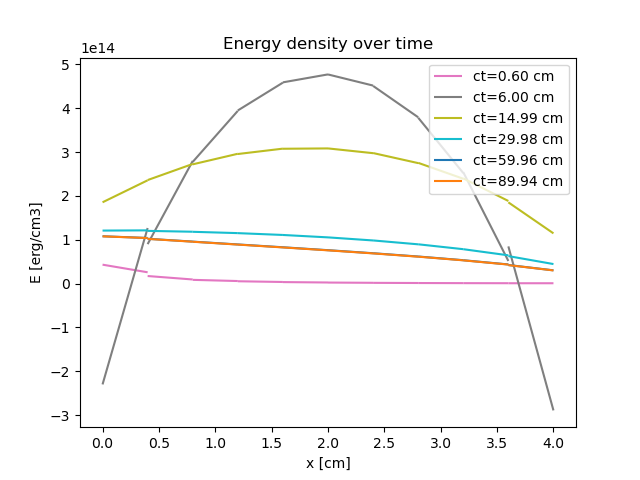
\includegraphics[width=\linewidth]{images/FC_energy_density.png}
        \caption{Energy Density}
    \end{subfigure}
    \begin{subfigure}{0.48\textwidth}
        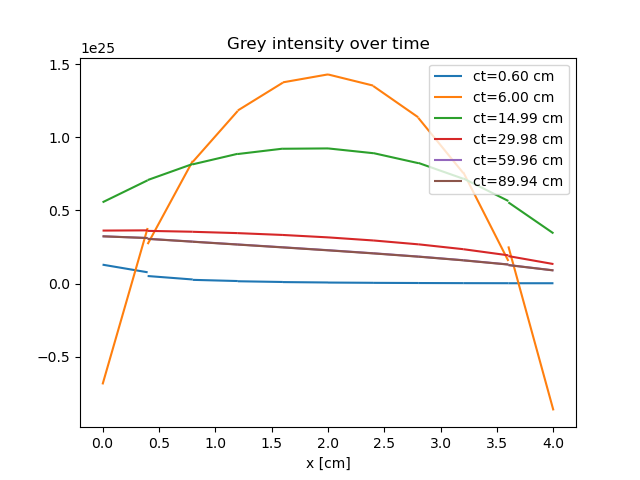
\includegraphics[width=\linewidth]{images/FC_grey_intensity.png}
        \caption{Grey Intensity}
    \end{subfigure}

    \begin{subfigure}[t]{0.48\textwidth}
        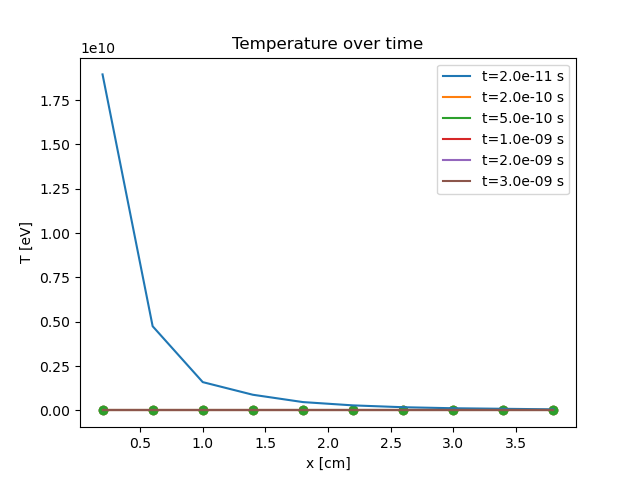
\includegraphics[width=\linewidth]{images/FC_temp_wide.png}
        \caption{Temperature, shown with FC IMC results (points)}\label{subfig:fc_temperature}
    \end{subfigure}
    \begin{subfigure}[t]{0.48\textwidth}
        \centering
        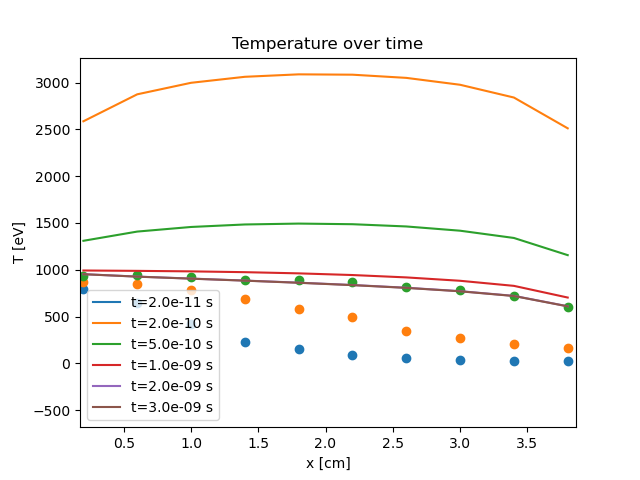
\includegraphics[width=\linewidth]{images/FC_temp_zoom.png}
        \caption{Temperature, cropped}
    \end{subfigure}
  \caption{Fleck and Cummings Test Results}\label{fig:FCresults}
\end{figure}


\begin{figure}[H]
  \centering
  \begin{subfigure}{0.48\textwidth}
        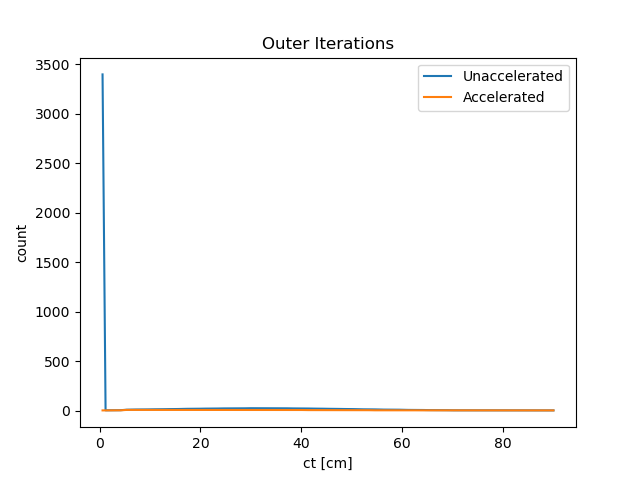
\includegraphics[width=\linewidth]{images/FC_outers.png}
        \caption{Outer Iterations}
    \end{subfigure}
    \begin{subfigure}{0.48\textwidth}
        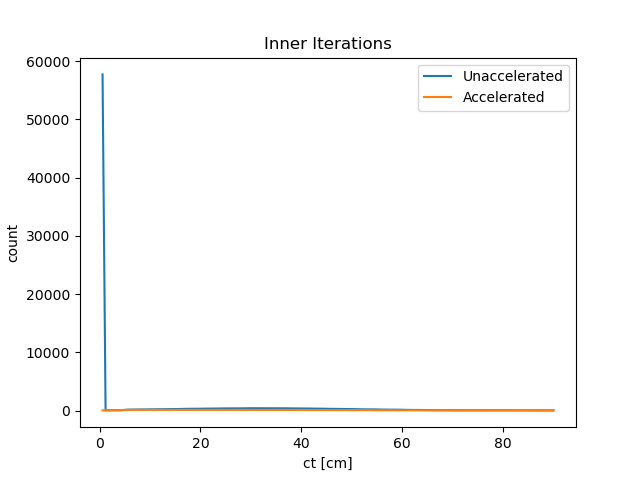
\includegraphics[width=\linewidth]{images/FC_inners.png}
        \caption{Inner Iterations}
    \end{subfigure}

    \begin{subfigure}[t]{0.48\textwidth}
        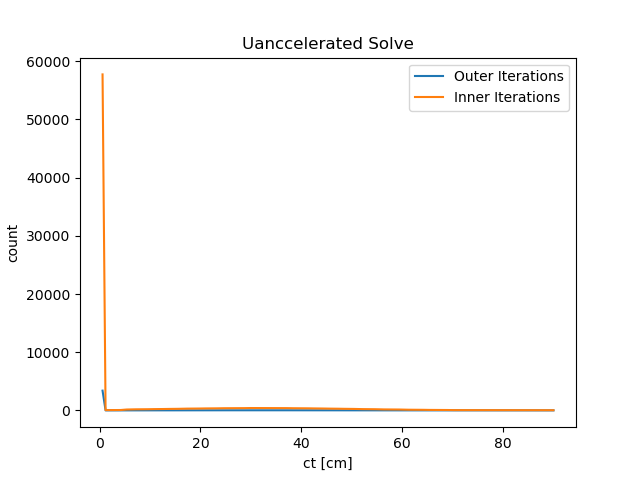
\includegraphics[width=\linewidth]{images/FC_unacc_iters.png}
        \caption{Unaccelerated Iterations}
    \end{subfigure}
    \begin{subfigure}[t]{0.48\textwidth}
        \centering
        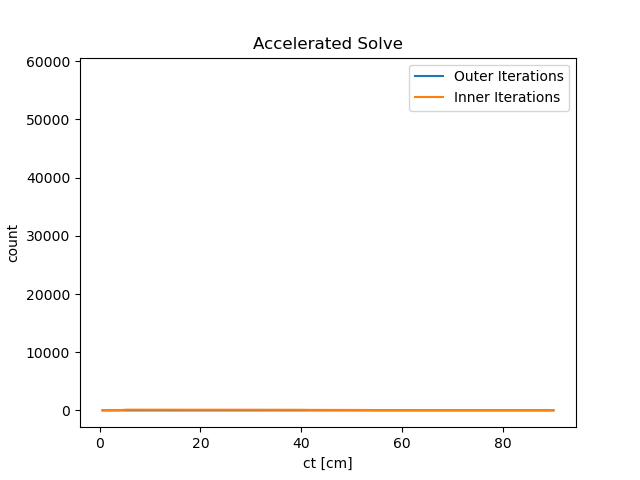
\includegraphics[width=\linewidth]{images/FC_accelerated_wide.png}
        \caption{Accelerated Iterations}
    \end{subfigure}

    \begin{subfigure}[t]{0.48\textwidth}
        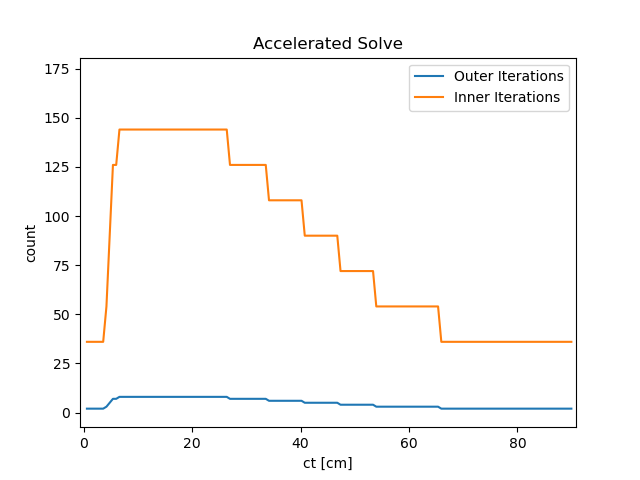
\includegraphics[width=\linewidth]{images/FC_accelerated_zoom.png}
        \caption{Accelerated Iterations (cropped)}
    \end{subfigure}
  \caption{Fleck and Cummings Test Iteration Results}\label{fig:FC_iters}
\end{figure}


The effects of these problems are not as strong when the initial temperature $T_b$ is high (i.e, the flux gradient and temperature changes are lower). Results for the same test where $T_b$ is set to $100$ eV are displayed in \autoref{fig:modifiedFC100}. Iterations are displayed in \autoref{fig:modifiedFC_iters}.


\begin{figure}[H]
  \centering
  \begin{subfigure}{0.48\textwidth}
        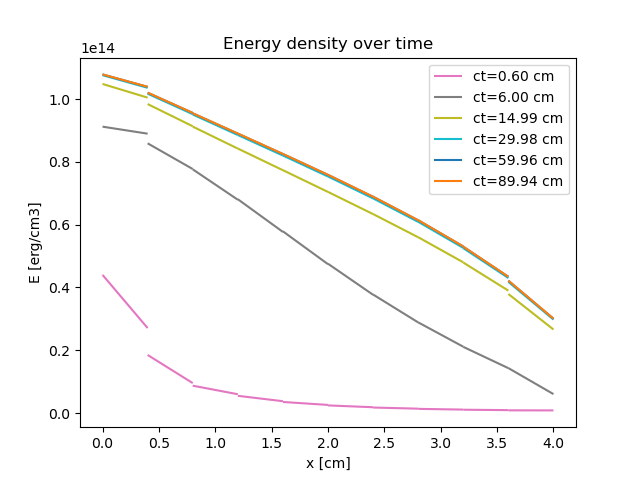
\includegraphics[width=\linewidth]{images/modifiedFC_energy_density.png}
        \caption{Energy Density}
    \end{subfigure}
    \begin{subfigure}{0.48\textwidth}
        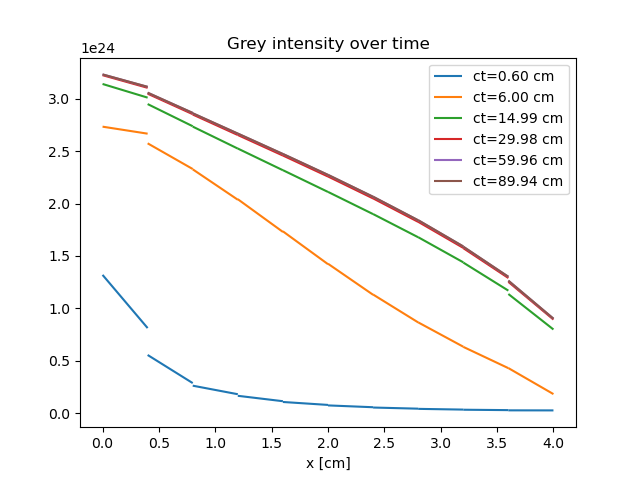
\includegraphics[width=\linewidth]{images/modifiedFC_grey_intensity.png}
        \caption{Grey Intensity}
    \end{subfigure}

    \begin{subfigure}{0.48\textwidth}
        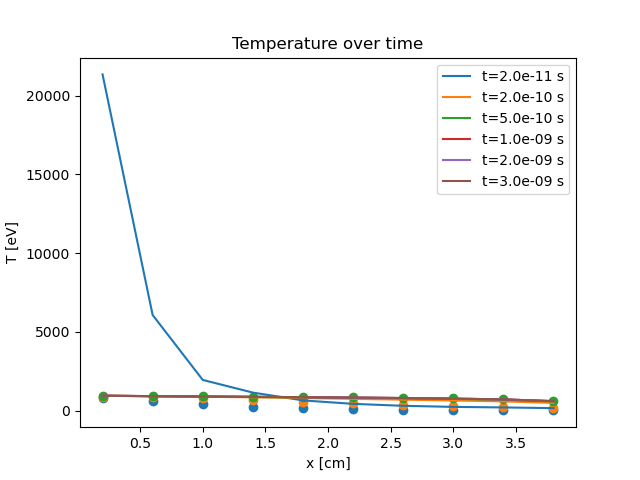
\includegraphics[width=\linewidth]{images/modfiedFC_temp_wide.png}
        \caption{Temperature}
    \end{subfigure}
    \begin{subfigure}{0.48\textwidth}
        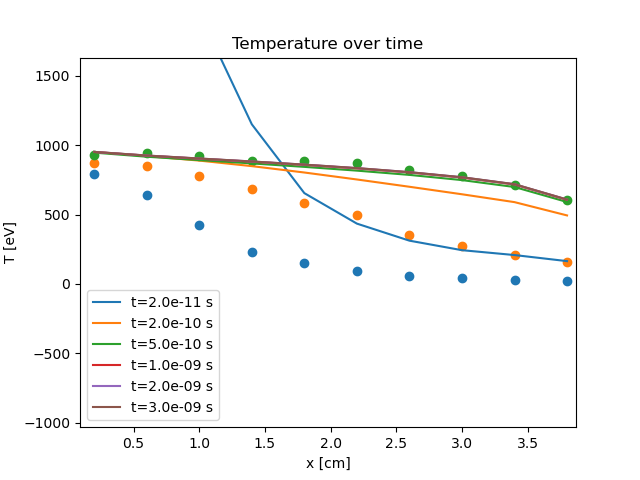
\includegraphics[width=\linewidth]{images/modfiedFC_temp_zoom.png}
        \caption{Temperature, cropped}
    \end{subfigure}
  \caption{Modified FC Test results with $T_b= 100$ eV}\label{fig:modifiedFC100}
\end{figure}

In both cases, the steady-state solution closely matches the IMC results~\cite{fleck1971implicit}, indicating that the basic transport solution method is correct, but that the issues are in the initial time steps, when the issues described in \autoref{sec:issues} cause the temperature, and thus the intensity solution, to blow up.

\begin{figure}[H]
  \centering
  \begin{subfigure}{0.48\textwidth}
        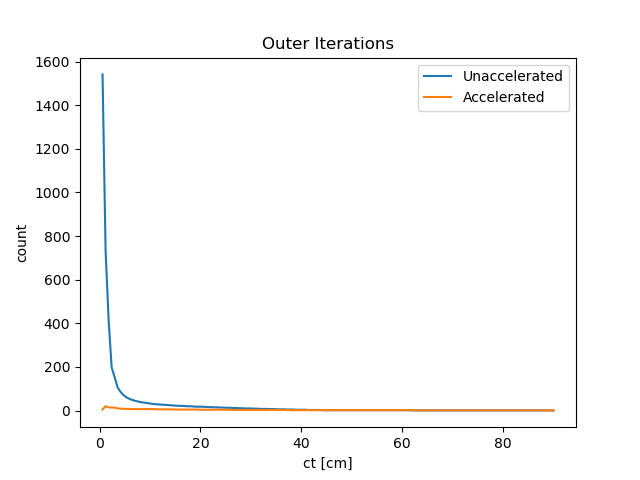
\includegraphics[width=\linewidth]{images/modifiedFC_outers.png}
        \caption{Outer Iterations}
    \end{subfigure}
    \begin{subfigure}{0.48\textwidth}
        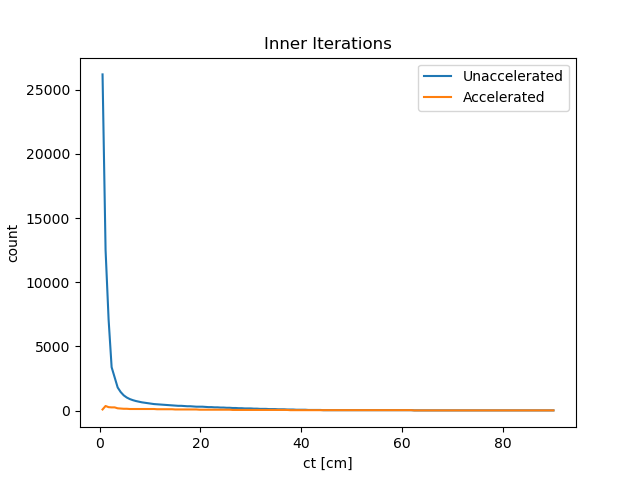
\includegraphics[width=\linewidth]{images/modifiedFC_inners.png}
        \caption{Inner Iterations}
    \end{subfigure}

    \begin{subfigure}[t]{0.48\textwidth}
        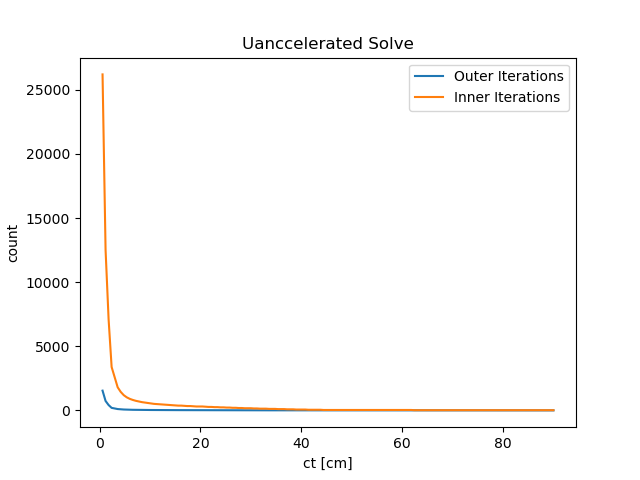
\includegraphics[width=\linewidth]{images/modifiedFC_unacc_iters.png}
        \caption{Unaccelerated Iterations}
    \end{subfigure}
    \begin{subfigure}[t]{0.48\textwidth}
        \centering
        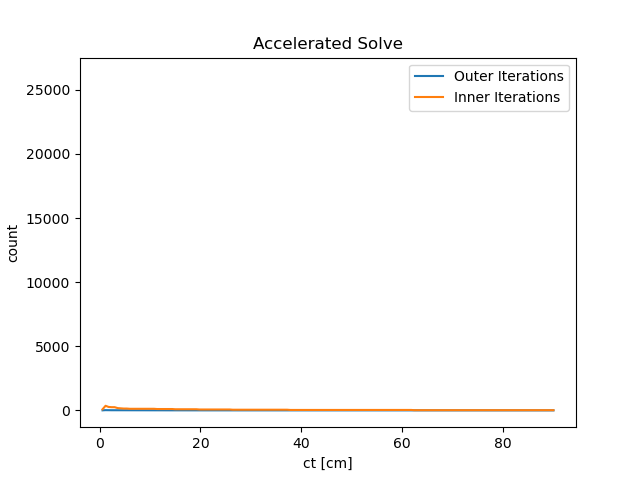
\includegraphics[width=\linewidth]{images/modifiedFC_accelerated_wide.png}
        \caption{Accelerated Iterations}
    \end{subfigure}

    \begin{subfigure}[t]{0.48\textwidth}
        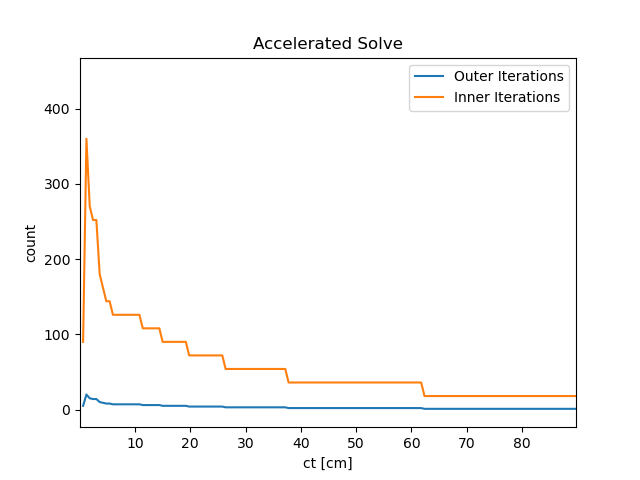
\includegraphics[width=\linewidth]{images/modifiedFC_accelerated_zoom.png}
        \caption{Accelerated Iterations (cropped)}
    \end{subfigure}
  \caption{Modified FC Test ($T_b = 100$ eV) Iteration Results}\label{fig:modifiedFC_iters}
\end{figure}


\section{Issues \& Next Steps} \label{sec:issues}

The unphysical results produced by the method as-is are due to the steep gradient present on the left boundary of the Fleck and Cummings test.

Two problems contribute to these results

\begin{enumerate}
    \item\label{item:gradient} The large gradient can lead to a negative energy density in the cell neighboring the boundary (see \autoref{fig:demo}). If this negative flux is low enough, it may cause the temperature in the next time step to become negative, in which case the Planck function is undefined and no further solution can be found.
    \begin{itemize}
        \item This issue may be solved either by implementing a negative temperature fix-up (set negative temperatures to some positive $\epsilon_T$) or by flux-limiting the diffusion solution.
    \end{itemize}
    \item\label{item:dbdt} The temperature change is implicit in the intensity calculation, using $\frac{\partial \beta}{\partial T}$, which is evaluated at the current time step. The actual value $\frac{\Delta \beta}{\Delta T}$ may be much different, especially at low temperatures where the magnitude of $\frac{\partial^2 \beta}{\partial T^2}$ is high (see \autoref{fig:dbdt_demo}). If the value of $\frac{\Delta \beta}{\Delta T}$ is too low, then the temperature change required to increase $\beta$ emission can be much too high; this is what causes the temperature blow-up in the Fleck and Cummings test (see \autoref{subfig:fc_temperature}).
    \begin{itemize}
        \item This issue may be addressed using Newton iteration to iteratively compute a more accurate $\frac{\Delta \beta}{\Delta T}$. This solution was explored in the code, but led to oscillatory iteration in some cases. The algorithm for this technique is shown in \autoref{alg:newton_lambda}.
    \end{itemize}
\end{enumerate}

Both of these issues are not relevant in the original report~\cite{morel1985synthetic}, where the method was developed and demonstrated for diffusive problems. The sample problem used to demonstrate the method was a small slab of iron, with an external heat source $Q$ which was switched on and off, where the solution is expected to have slow temperature changes and no steep gradients in the intensity solution; neither of these features are true for the Fleck and Cummings test.


\begin{algorithm}
    \caption{Unaccelerated Algorithm using Newton Iteration for Implicit Temperature}\label{alg:newton_lambda}
  \begin{algorithmic}[0]
    % \Require{$x$ and $y$ are packed dna strings of equal length $n$}
    \Statex{}
    \While{$t^n \leq t^{end}$}
      \Let{$n$}{$n+1$}
      \State{Compute (lagged) temperature-dependent coefficients using $T\vert_{t=t^{n-1}}$}
      \State{Compute initial $\lambda = \frac{\partial \beta}{\partial T}\vert_{t=t^{n-1}}$}

    \While{$|\lambda^{(i)} - \lambda^{(i-1)}| > \epsilon_\lambda |\lambda^{(i-1)}|$}
        \Let{$i$}{$i+1$}
        \While{$\norm{I^{(l)} - I^{(l-1)}} > \epsilon_c\norm{I^{(l-1)}}$}
        \Let{$l$}{$l+1$}
        \Let{$I_k^{(l+1/2)}$}{Source iteration on $\eta\chi_k \sum_{g=1}^{N_g}\sigma_{f, g}I_g^{n+1}$ (\ref{eq:iterative_neutron}), using $\beta^n \approx \beta^{n-1} + \lambda^{(i)} \Delta T$}
        \Let{$I_k^{n}$}{$I_k^{(l+1)}$}
        \EndWhile{}
        \Let{$\lambda^{(i)}$}{$\frac{\beta^{(n+1)} - \beta^{(n)}}{T^{(n+1)} - T^{(n)}}$}
    \EndWhile{}
      \While{$\norm{I^{(l)} - I^{(l-1)}} > \epsilon\norm{I^{(l-1)}}$}
        \Let{$l$}{$l+1$}
        \Let{$I_k^{(l+1/2)}$}{Source iteration on $\eta\chi_k \sum_{g=1}^{N_g}\sigma_{f, g}I_g^{n+1}$ (\ref{eq:iterative_neutron}), using $\beta^n \approx \beta^{n-1} + \lambda \Delta T$}
      \EndWhile{}
      \Let{$I_k^{n}$}{$I_k^{(l+1)}$}
      \State{Recover $\Delta T^{n+1/2}$ from $I_k^{n}$ (\ref{eq:temperature-change})}
      \If{$K \neq 0 \land u \neq 0$}
        \State{Solve thermal diffusion equation for $\Delta T^{n+1}$}
      \EndIf{}
      \Let{$T^{n+1}$}{$T^n + \Delta T^{n+1/2} + \Delta T^{n+1}$}
    \EndWhile{}
  \end{algorithmic}
\end{algorithm}



\begin{figure}[H]
    \centering
    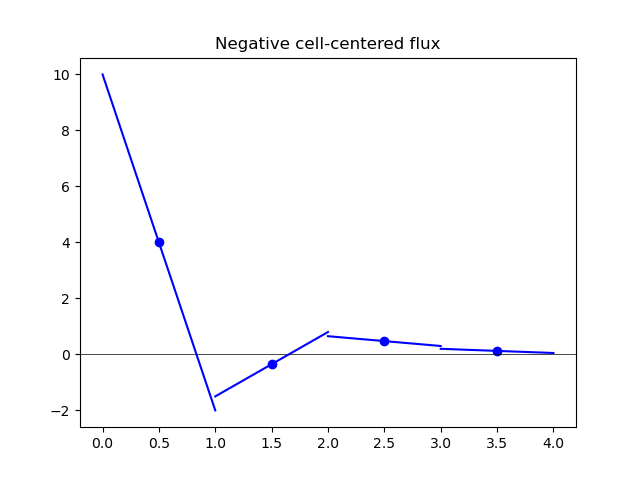
\includegraphics[width=0.65\linewidth]{images/demo.png}
    \caption{Negative flux illustration}\label{fig:demo}
\end{figure}


\begin{figure}
    \centering
    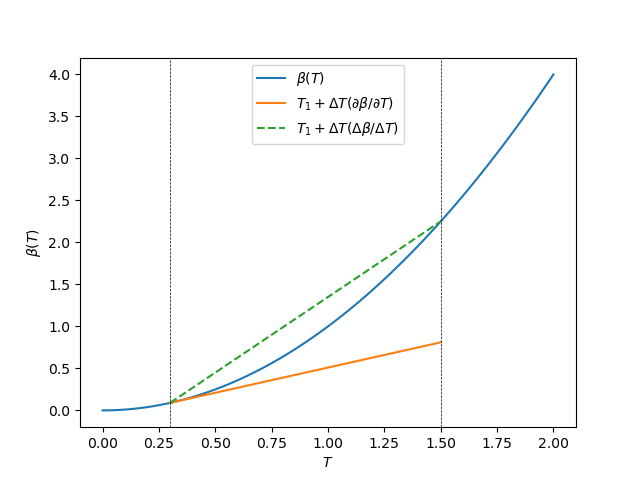
\includegraphics[width=0.65\linewidth]{images/dbdt_demo.png}
    \caption{Illustration of $\frac{\Delta \beta}{\Delta T}$}\label{fig:dbdt_demo}
\end{figure}




\newpage

\appendix

\section{Python Functions}\label{sec:tree}

\newcommand{\descript}[1]{\dotfill \begin{minipage}[t]{5cm} #1 
\end{minipage}\hspace{2.5cm}}

\dirtree{%
    .1 /.
    .2 method\DTcomment{All iteration, acceleration}.
    .3 assemble\_global\_matrix()\descript{Assemble global LD FEM matrix}.
    .3 get\_HO\_source() \descript{for group $k$, compute fission source, time differencing source, external source, and add boundary conditions}.
    .3 get\_LO\_source().
    .3 assemble\_HO()\descript{Compute global matrix and source, assemble into class}.
    .3 assemble\_LO().
    .3 unaccelerated\_loop()\descript{For a single time step. Call assemble\_HO and solve system until convergence is reached}.
    .3 accelerated\_loop()\descript{Same as unaccelerated\_loop(), but includes grey correction term. Assemble and solve HO system, compute grey coefficients, solve grey system, get corrected iterate, until convergence}.
    .3 loop()\descript{Read flags and call appropriate ...loop()}.
    .3 update\_temperature()\descript{\autoref{eq:temperature-change}}.
    .3 solve\_diffusion()\descript{handles time advancement. At each time step, call loop(), record results}.
    .2 tools\DTcomment{Data classes, plotting tools, local matrices}.
    .3 B\_1, B\_2, M, M\_wide\descript{Local LD matrices}.
    .3 dbl()\descript{Repeat mesh.nx array to be 2*mesh.nx. Prepares piecewise constant values (opacity, temperature, etc) for use in LD solution}.
    .3 Transport\_solution\descript{Contains intensity and flux}.
    .3 Discretization\descript{Contains discretization parameters dt, dx, group structure, etc, and constants for computational units}.
    .3 Global\_system\descript{Global matrix and source vector}.
    .3 MG\_coefficients \descript{$\sigma_k, \eta, \chi_k, \frac{\partial \beta}{\partial T}, \beta_k, D_k, S_k, \varkappa_k$}.
    .3 Grey\_coeff\descript{$\langle D \rangle, \langle \sigma_f \rangle, \langle \sigma_t \rangle, r$}.
    .3 LD\_plottable\descript{Prepares LD solution for plotting}.
    .3 plot\_LD\_groups().
    .3 plot\_LD\_grey().
    .2 physics\DTcomment{Physical constants, Planck Function and derivative}.
    .3 cumulative\_sigma()\descript{Group Stefan-Boltzmann constant}.
    .3 group\_planck()\descript{Grouped Planck spectrum}.
    .3 cumulative\_dsigma\_dt().
    .3 group\_db\_dt().
}





\bibliographystyle{ieeetr}
\bibliography{references.bib}


\end{document}